\documentclass[12pt]{article}
\usepackage{a4wide}
\usepackage[utf8]{inputenc}
\usepackage[T1]{fontenc}
\usepackage[english]{babel}
\usepackage{times}
\usepackage{graphicx}
\usepackage{url}
\usepackage{color}
\usepackage{xspace}
\usepackage{amssymb}
\usepackage{amsmath}


\newcommand{\stCode}[1]{\textsf{#1}\xspace}
\newcommand{\st}[1]{\stCode{#1}}

\newcommand{\stMethod}[1]{\textsf{#1}}
\newcommand{\sep}{\texttt{>>}\xspace}
\newcommand{\stAssoc}{\texttt{->}\xspace}



\newcommand{\stBar}{$\mid$}
%\newcommand{\stSelector}{$\gg$}
\newcommand{\stSelector}[1]{{\textsf{\##1}}\xspace}



\newcommand{\ret}{\^{}}
\newcommand{\msup}{$>$}
%\newcommand{\ret}{$\uparrow$\xspace}

\newcommand{\myparagraph}[1]{\noindent\textbf{#1.}}
\newcommand{\eg}{\emph{e.g.,}\xspace}
\newcommand{\ie}{\emph{i.e.,}\xspace}
\newcommand{\ct}[1]{{\textsf{#1}}\xspace}

\usepackage{alltt}
\newenvironment{code}
    {\begin{alltt}\sffamily\small}
    {\end{alltt}\normalsize}

\newcommand{\infe}{$<$}
\newcommand{\supe}{$\rightarrow$\xspace}
\newcommand{\di}{$\gg$\xspace}



\newcommand{\zoneReponse}[2]{\fbox{\parbox{\textwidth}{#2\hspace*{\textwidth}\vspace*{#1}}}}

\newenvironment{encadre}{%
\begin{minipage}{0.89\columnwidth}%
}{%
\end{minipage}
}

\begin{document}
\vspace*{-3.5cm}
\zoneReponse{1.5cm}{{\bf Nom-Prénom : }}

\begin{center}
{\it\Large Programmation par Objets}\\[0.25cm]
{\Large\bf Devoir surveillé}\\[0.25cm]
{\em\bf Durée : 15 min}
\end{center}

\paragraph{Consignes:}
Les réponses aux exercices doivent être faites sur le présent sujet qui doit être rendu au professeur.
L'utilisation des ordinateurs est autorisée.


\section{Soit la classe \st{Personne} telle que}

\begin{itemize}
	\item Une personne a un nom (une chaîne de caractère), un père et une mère, elles-mêmes instances de la classe \st{Personne} ou \st{nil} si elles sont inconnus (non initialisés).
	\item Une personne répond au message \st{nom: unNom}, qui mémorise le paramètre comme le nom de la personne.
	\item Une personne répond au message \st{pere: unePersonne}, qui mémorise le paramètre comme le père de la personne.
	\item Une personne répond au message \st{mere: unePersonne}, qui mémorise le paramètre comme la mère de la personne.	
	\item Une personne répond au message \st{nom} en retournant le nom de la personne.
	\item Une personne répond au message \st{pere} en retournant le père de la personne.
	\item Une personne répond au message \st{mere} en retournant la mère de la personne.
\end{itemize}

\subsection{Donnez la définition de la classe Personne}
\zoneReponse{5cm}

\subsection{Analysez le code ci-dessous qui est évalué dans un \emph{workspace}}
\begin{code}
	eric := Personne new.
	eric nom: 'Eric'.
	valerie := Personne new.
	valerie nom: 'Valerie'
	charlotte := Personne new.
	charlotte nom: 'Charlotte'.
	charlotte pere: eric.
	charlotte mere: valerie.
	fred := Personne new.
	fred nom: 'Fred'.
	eric := fred.
\end{code}
Quel est le resultat de l'expression \st{charlotte pere nom} ?\~\\

\zoneReponse{2cm}

\subsection {Donnez la définition de la méthode \st{parents} qui retourne une collection qui regroupe les deux parents du receveur. La collection ne doit comporter que les parents connus (différents de \st{nil})}
	\zoneReponse{6cm}

\subsection {La méthode \st{ancetres} qui retourne  une collection qui regroupe toutes les personnes de l'arbre généalogique}
	\zoneReponse{6cm}

\section{Soit un jeu de Tetris composé des classes suivantes}
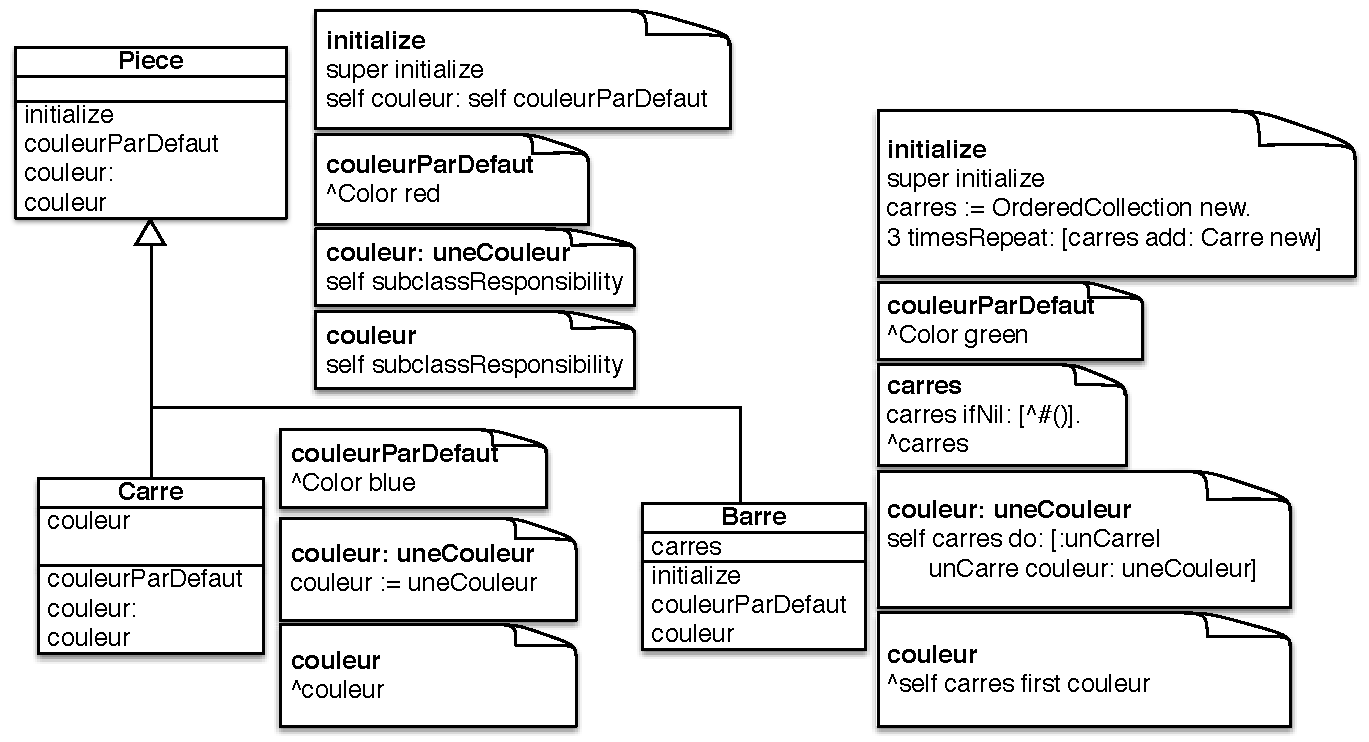
\includegraphics[width=\textwidth]{heritage}
Quel est le résultat de l'expression \st{Barre new couleur}\\
\zoneReponse{2cm}

\end{document}